\newpage


\section{Hyper-parameters}\label{sec:hyper-parameters}

Proposed genetic algorithm~\ref{alg:genetic} has eight hyperparameters.
They are described in table~\ref{tab:hyperparameters-description}.
The rest of the sections discuss these hyperparameters further and tries to find their reasonable values.

Hyperparameter testing is performed by changing only the hyperparameter under test.
Hyperparameters not under test are identical to the values in listing~\ref{lst:computation-submission-dataset}.
The exceptions are penalization constants $\lambda, \gamma$ (eq.~\ref{eq:objective}), and \verb|populationSize|.
Penalization constants are set to the length of the layout diagonal (see~\ref{subsec:overlapping-penalization-constant}).
Population size is set to $50N$, where $N$ is the size of the instance.
The reason for choosing such parameters as base parameters for testing
is preliminary results (not presented in this thesis), which proved correct in many cases.

To achieve the statistical significance of the results presented in this section, each computation (sec.~\ref{sec:implementation}) is submitted five times with a different random seed.
Presented values are thus an average from five samples.


\begin{table}[h!]
    \caption{Hyperparameters of the genetic algorithm}
    \label{tab:hyperparameters-description}
    \begin{tabular}{lc}
        \hline
        \multicolumn{1}{c}{\textbf{hyperparameter}} & \textbf{description}                                       \\ \hline
        \verb|maxNumberOfIter|                      & maximum number of iterations                               \\ \hline
        \verb|populationSize|                       & population size                                            \\ \hline
        \verb|maximumWildCardCount| & \begin{tabular}[c]{@{}c@{}}
                                          limit on the maximum number of $*$ cut types\\ produced by $OR_{prob}$ decoding
        \end{tabular} \\ \hline
        \verb|orientationWeights|                   & penalization vector $P$ from eq.~\ref{eq:crossover-orprob} \\ \hline
        \verb|populationDivisionCounts| & \begin{tabular}[c]{@{}c@{}}
                                              reproductive plan ratios\\ (left part of fig.~\ref{fig:population-schema})
        \end{tabular} \\ \hline
        \verb|initialPopulationDivisionCounts| &
        \begin{tabular}[c]{@{}c@{}}
            initial population ratios\\ (right part of fig.~\ref{fig:population-schema})
        \end{tabular} \\ \hline
        \verb|overlappingPenalizationConstant| &
        \begin{tabular}[c]{@{}c@{}}
            overlapping paintings penalization\\ parameter $\lambda$ from eq.~\ref{eq:objective}
        \end{tabular} \\ \hline
        \verb|outsideOfAllocatedAreaPenalizationConstant| &
        \begin{tabular}[c]{@{}c@{}}
            outside of allocated area penalization\\ parameter $\gamma$ from eq.~\ref{eq:objective}
        \end{tabular} \\ \hline
    \end{tabular}
\end{table}

\subsection{Max number of iter}\label{subsec:max-number-of-iter}
Results for hyperparameter \verb|maxNumberOfIter| are in figure~\ref{fig:hyperparameters-max-number-of-iter}.
We can see the initial decrease of the average population objective for both random instances.
Between iterations 100 and 150, decreasing trend and fluctuations stop.

The conclusion is that at least 150 iterations are needed before the average population objective
stops decreasing rapidly.

\subsection{Population size}\label{subsec:population-size}

Population size is calculated as $kN$, where $k$ is \definice{population scaling factor}
and $N$ is instance size.
Thus, the population size is linear with respect to the instance size.

Results for two random instances are in figure~\ref{fig:hyperparameters-population-size}.
We can see that scaling factor $10$ does not allow
the population objective average to decrease to the levels comparable to scaling factors $50$ and $100$.
It might imply that the scaling factor $10$ cannot represent knowledge gathered over time
in the genetic algorithm or that more iterations are needed.

The conclusion is that using scaling factor between $50$ and $100$ is sufficient, with bias towards $100$
for obtaining better average objective performance.
However, increasing the scaling factor leads to slower computation speed as every population contains
more individuals for which genetic operators and reproductive plan must be computed.

\subsection{Maximum wild card count}\label{subsec:maximum-wild-card-count}
Hyperparameter \verb|maximumWildCardCount| limits the maximum number of $*$ cut types produced by $OR_{prob}$ decoding (subsec.~\ref{subsec:individual-decoding}).
It is recommended to keep this hyperparameter very low or even set it to zero.
The reason is that if it is high, computation time increases as $*$ spreads in the population.
For example, consider an individual whose orientation vector is solely composed of $*$ cut types.
If the size of that vector is $n$, individual decodes to $2^n$ resolved slicing trees as seen in figure~\ref{fig:layout-construction-steps}.


Results for two random instances are in figure~\ref{fig:hyperparameters-maximum-wild-card-count}.
\todo{popsat vysledky az dobehnou vypocty}Maecenas libero. Lorem ipsum dolor sit amet, consectetuer adipiscing elit. Nunc dapibus tortor vel mi dapibus sollicitudin. Duis viverra diam non justo. Integer rutrum, orci vestibulum ullamcorper ultricies, lacus quam ultricies odio, vitae placerat pede sem sit amet enim.

The conclusion is ...

\subsection{Orientation weights}\label{subsec:orientation-weights}
Hyperparameter \verb|orientationWeights| determines the bias towards the type of cut ($H$, $V$, $*$, see~\ref{subsec:individual-decoding}) \textit{during crossover}.
The orientation penalization vector $P$ from eq.~\ref{eq:crossover-orprob} contains the penalization value for each cut type.
In this thesis, only penalization for the wildcard cut type $*$ is tested, as there is no need to penalize or have a preference for $H$ or $V$ cut types.
Recall that the hyperparameter \verb|maximumWildCardCount| is \textit{set to one}, as described at the beginning of the section and showed in listing~\ref{lst:computation-submission-dataset}.

Performance results for two random instances are in figure~\ref{fig:hyperparameters-orientation-weights}.
We can see that for random\_10 instance,
weight does not significantly influence the average population objective, and after iteration 250, differences become negligible.
However, for random\_20 instance,
weight one (no penalization) has a faster-decreasing trend and produces a population with a better average population objective.

First conclusion it that (a) smaller instances, such as random\_10, do not benefit from the introduction of wildcard cut type $*$,
and (b) bigger instances, such as random\_20, benefit from no penalization by having a faster-decreasing trend and producing a better average population.

The reason for better average performance at larger instance with weight one (no penalization) might
be that search space increases exponentially (there are at least $2^{N-1}$ different unresolved slicing trees for instance of size $N$) and the introduction of wildcard cut type $*$ starts to manifest itself
at larger instances.

Results for the number of wildcard cut types $*$ at the best individual at each iteration are in
figure~\ref{fig:hyperparameters-orientation-weights-wildcard-cut-type-spread}.
We can see that for the random\_10 instance, weights below one have less than one wildcard on average.
However, on average, there are between three and four wildcards for a weight equal to one (no penalization).
Similar can be seen for random\_20 instance.

Second conclusion is that if we want to be certain that wildcard cut type $*$ is contained in the best individual at each iteration,
wild card orientation weight must be set close to one.

The reason why there are wildcards present in the figure~~\ref{fig:hyperparameters-orientation-weights-wildcard-cut-type-spread}
even for weight equal to zero (maximal penalization) is that wildcard can be introduced to a chromosome by mutation
or injection random individuals (see reproductive plan~\ref{subsec:reproductive-plan}).
Penalization described only applies to the crossover.

\subsection{Population division counts}\label{subsec:population-division-counts}
Hyperparameter \verb|populationDivisionCounts| configures ratios in the reproductive plan (subsec.~\ref{subsec:reproductive-plan}).
It influences how the next generation is created in the genetic algorithm~\ref{alg:genetic}
by setting (a) how many elite individuals are copied, (b) how many children are created using a crossover operator,
(c) how many mutants are created using a mutation operator, (d) how many tournament winners are included,
and (e) how many random individuals are injected.

Performance results for two random instances are in figure~\ref{fig:hyperparameters-population-division-counts}.
Removing the injection of $0.1$ random individuals achieves a better average population objective for both instances.
The reason for that might be the implementation of crossover and that offsprings created by crossover
are the major part of the next population.
Crossover implementation (described in subsec.~\ref{subsec:crossover}) uses weights $w_A$ and $w_B$
based on the performance of parents $A$ and $B$.
Weights limit the transfer of information from the lower-performance parent.
However, consider the weights are almost the same, i.e., parents perform similarly, and each parent represents a different (sub)-optimal solution. Information transfer does not happen in that case, and the offspring performs poorly.
It stems from the idea that each individual contains stochastic vectors that approximate the probability mass
function, and if each parent represents a different but performant function, the offspring contains
neither of those performant probability mass functions.

The conclusion is that parents with similar performance representing different (sub)-optimal solution
produce offspring that perform poorly.
It might also be the reason why the second-best result in figure~\ref{fig:hyperparameters-population-division-counts}
is achieved by, in addition to removing random individuals, also removing the elitism strategy.
Elitism keeps track of any (sub)-optimal solutions, which are then used as a first parent
to the crossover (right part of fig.~\ref{fig:population-schema}).
Thus, elitism increases the probability that crossover parents represent different (sub)-optimal solutions.

\subsection{Initial population division counts}\label{subsec:initial-population-division-counts}
Hyperparameter \verb|initialPopulationDivisionCounts| configures generation ratios of the initial population (left part of fig.~\ref{fig:population-schema}).
It consists of randomly generated and greedily generated individuals.

Performance results for two random instances are in figure~\ref{fig:hyperparameters-initial-population-division-counts}.
We can see that results for the different ratios does not significantly differ.

Conclusion is that hyperparameter Hyperparameter \verb|initialPopulationDivisionCounts| does not play a significant role in the obtained results.

\subsection{Overlapping penalization constant}\label{subsec:overlapping-penalization-constant}

It is not desirable to produce painting placement solutions that overlap.
Thus, hyperparameter \verb|overlappingPenalizationConstant| penalizes
individuals representing such a solution.

The optimal value must be strong enough to remove or limit overlapping solutions from the population.
Also, it must be low enough not to become the dominant part of the objective function (eq.~\ref{eq:objective})
as it can lead the genetic algorithm to neglect other parts – eval function, clustering, and flow between paintings.

Values tested for \verb|overlappingPenalizationConstant| are proportional to the diagonal
length of the layout to which paintings are placed.
It means that if we define constant $k$, width of the layout as $W$ and its height as $H$,
tested value is $k\sqrt{W^2 + H^2}$.

Results are in figure~\ref{fig:overlapping-penalization} for two instances.
From it, we can deduce that the optimal value for \textit{overlapping penalization constant} is between $2$ and $5$ times the length of the layout diagonal.

\subsection{Outside of allocated area penalization constant}\label{subsec:outside-of-allocated-area-penalization-constant}
TODO

\afterpage{%
    \clearpage% Flush earlier floats (otherwise order might not be correct)
    \begin{landscape}% Landscape page
        \begin{figure}
            \centering
            \subfloat{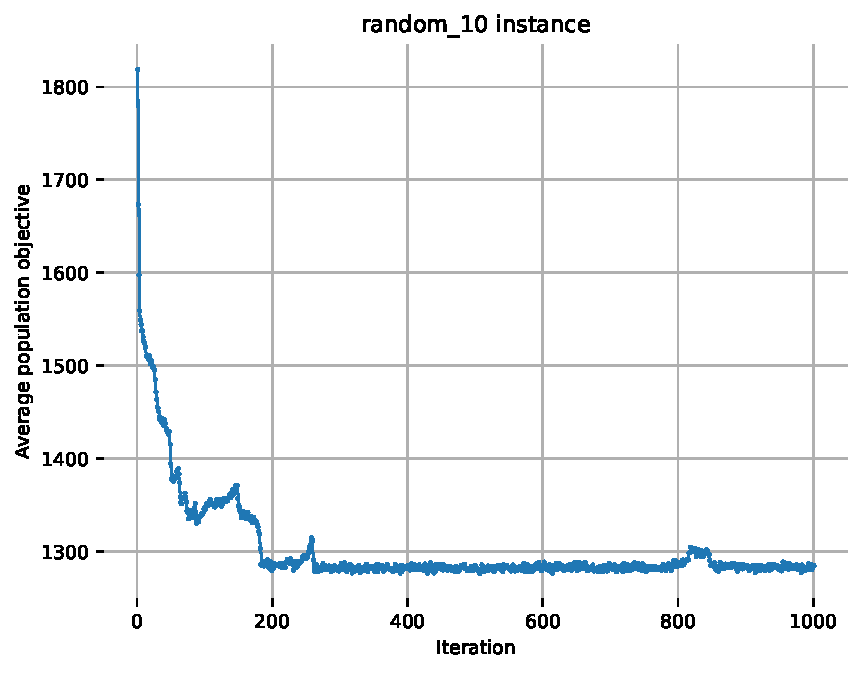
\includegraphics[width=0.8\textwidth]{hyperparameters/max_number_of_iter_random_10}\label{subfig:hyperparameters-max-number-of-iter-random-10}}
            \subfloat{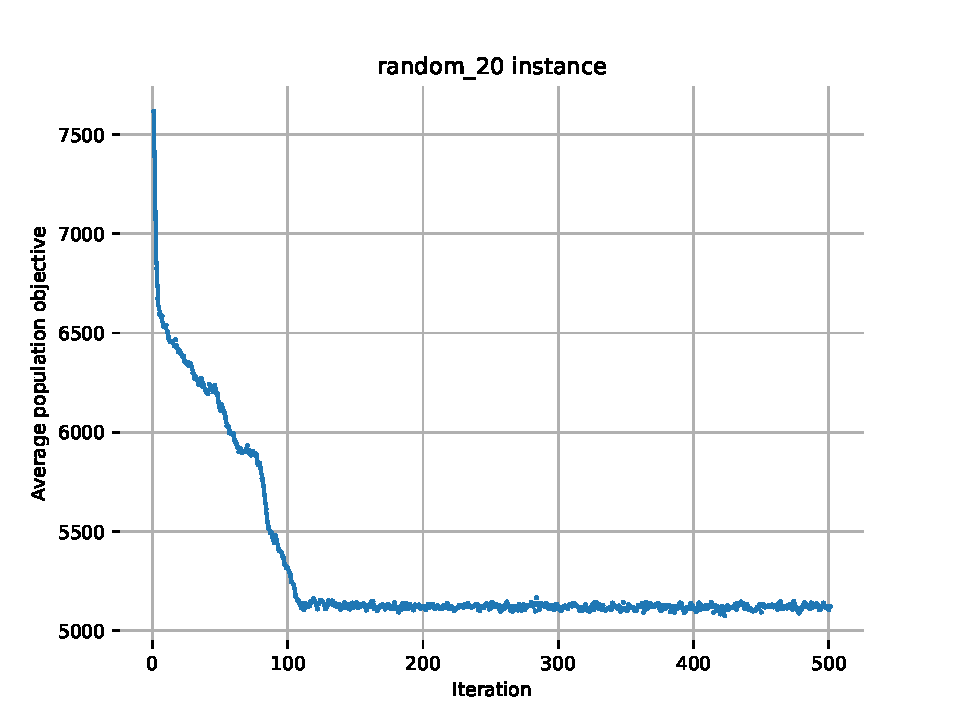
\includegraphics[width=0.8\textwidth]{hyperparameters/max_number_of_iter_random_20}\label{subfig:hyperparameters-max-number-of-iter-random-20}}
            \caption[Testing maximum number of iterations]
            {Testing maximum number of iterations at two random instances.}
            \label{fig:hyperparameters-max-number-of-iter}%
        \end{figure}
    \end{landscape}
    \clearpage% Flush page
}


\afterpage{%
    \clearpage% Flush earlier floats (otherwise order might not be correct)
    \begin{landscape}% Landscape page
        \begin{figure}
            \centering
            \subfloat{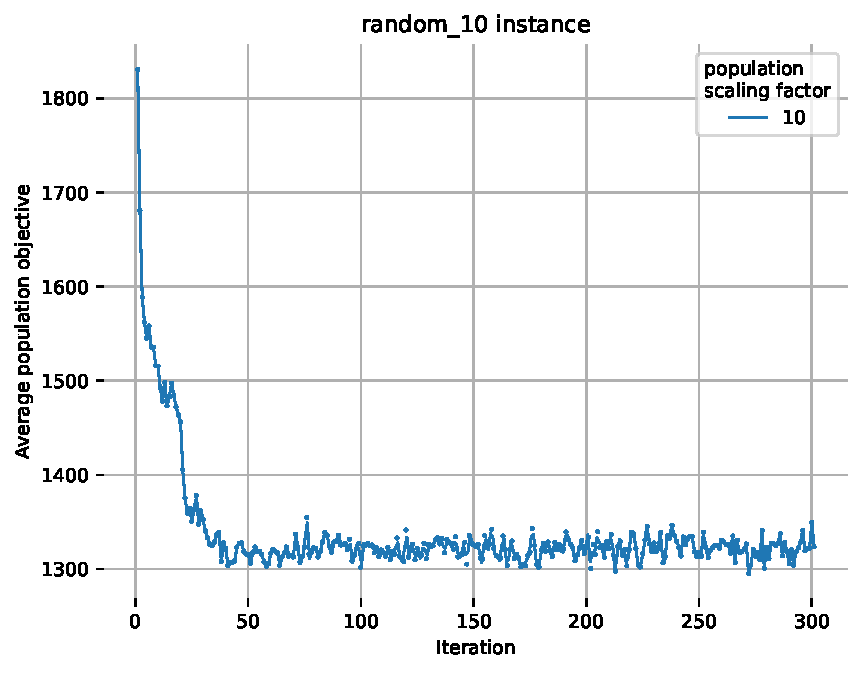
\includegraphics[width=0.8\textwidth]{hyperparameters/population_size_random_10}\label{subfig:hyperparameters-population-size-random-10}}
            \subfloat{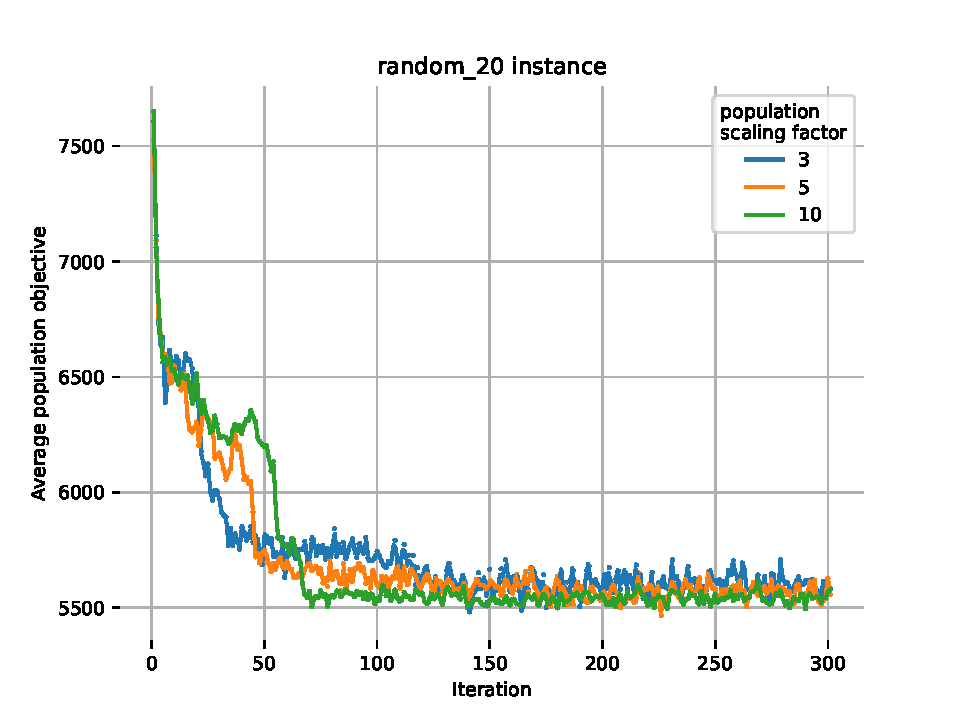
\includegraphics[width=0.8\textwidth]{hyperparameters/population_size_random_20}\label{subfig:hyperparameters-population-size-random-20}}
            \caption[Testing population scaling factor]
            {Testing population scaling factor at two random instances.
            The population size is $kN$ for population scaling factor $k$ and instance of size $N$. }
            \label{fig:hyperparameters-population-size}%
        \end{figure}
    \end{landscape}
    \clearpage% Flush page
}


%\afterpage{%
\clearpage% Flush earlier floats (otherwise order might not be correct)
%    \begin{landscape}% Landscape page
\begin{figure}
    \centering
    \subfloat{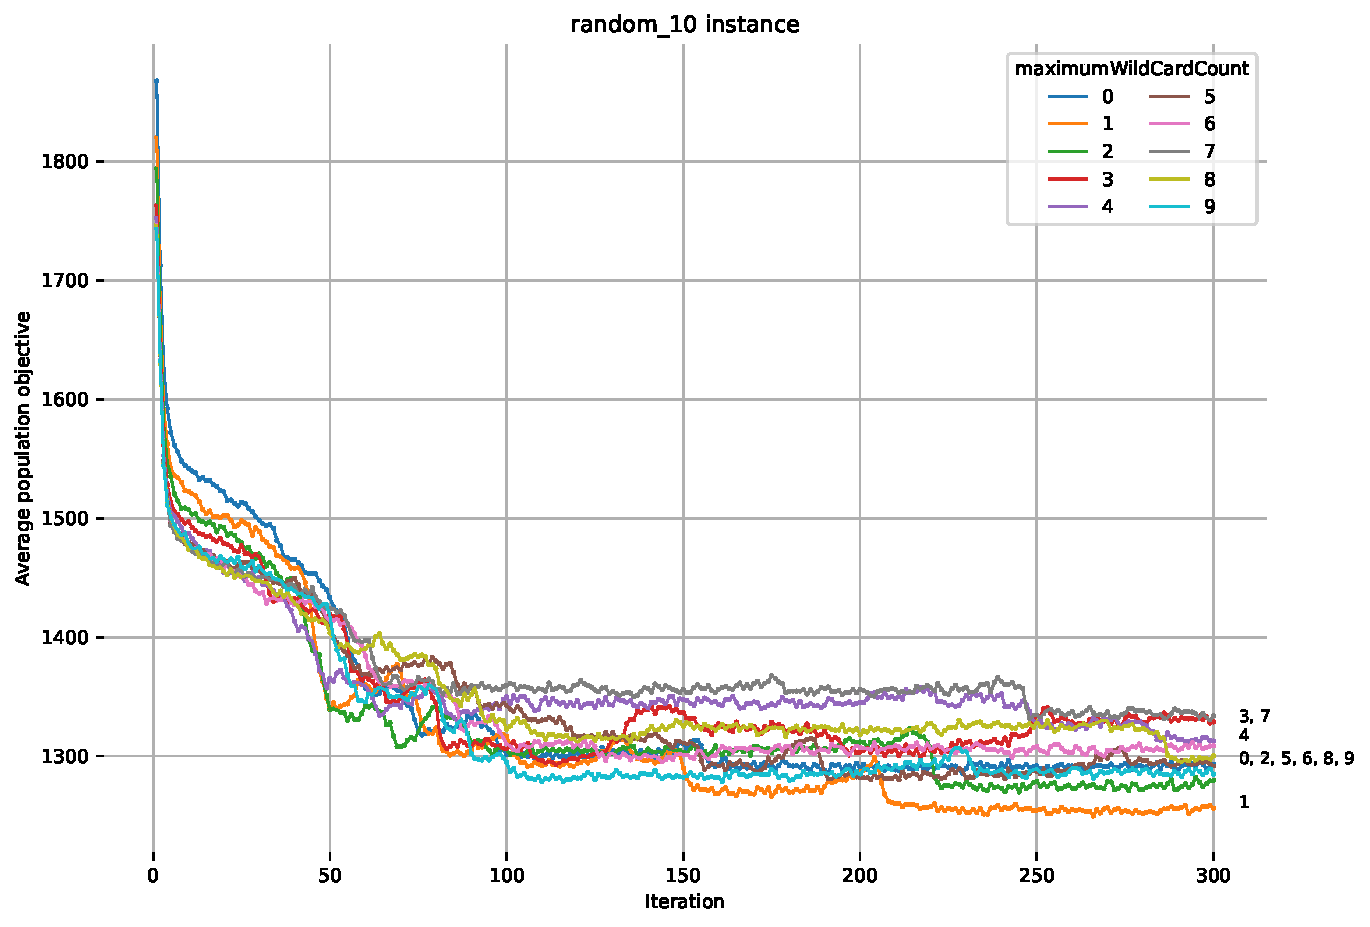
\includegraphics[width=1.1\textwidth]{hyperparameters/maximum_wild_card_count_performance_random_10}\label{subfig:hyperparameters-maximum-wild-card-count-performance}}

    \subfloat{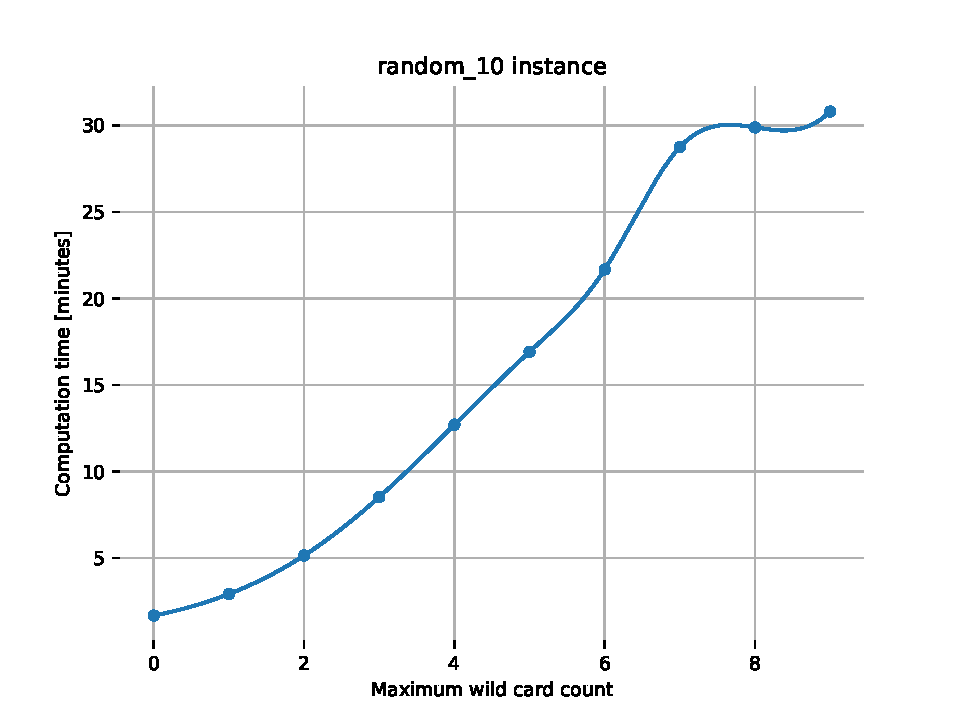
\includegraphics[width=0.8\textwidth]{hyperparameters/maximum_wild_card_count_computation_time_random_10}\label{subfig:hyperparameters-maximum-wild-card-count-computation-speed}}
    \caption[Testing maximum wild card count]
    {Testing increasing maximum wild card count. Performance (top) and computation speed (bottom).}
    \label{fig:hyperparameters-maximum-wild-card-count}%
\end{figure}
%    \end{landscape}
%    \clearpage% Flush page
%}


%\afterpage{%
%    \clearpage% Flush earlier floats (otherwise order might not be correct)
%    \begin{landscape}% Landscape page
\begin{figure}
    \centering
    \subfloat{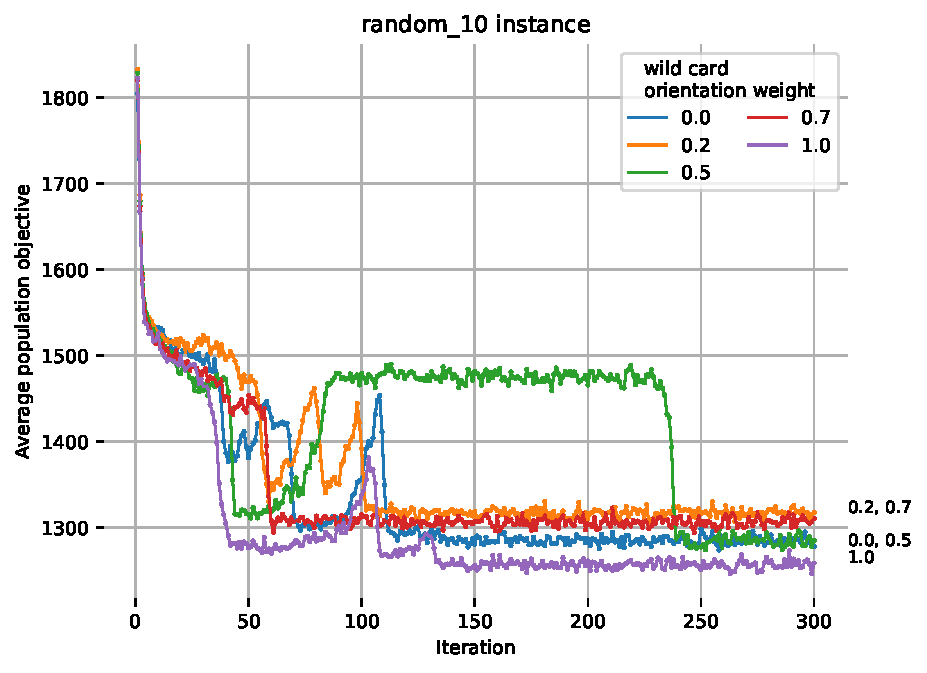
\includegraphics[width=1.1\textwidth]{hyperparameters/orientation_weights_random_10}\label{subfig:hyperparameters-orientation-weights-random-10}}

    \subfloat{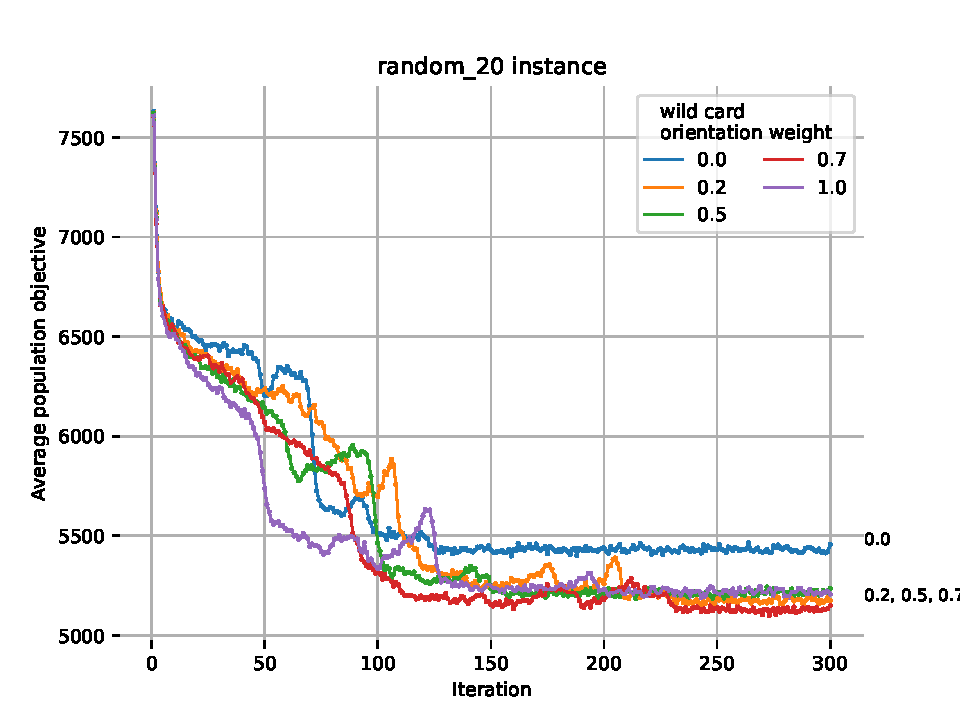
\includegraphics[width=1.1\textwidth]{hyperparameters/orientation_weights_random_20}\label{subfig:hyperparameters-orientation-weights-random-20}}
    \cprotect\caption[Testing orientation weights performance]
    {Testing performance of orientation weight for a wildcard cut type $*$ at two random instances.
    Hyperparameter \verb|maximumWildCardCount| is 1.}
    \label{fig:hyperparameters-orientation-weights}%
\end{figure}
%    \end{landscape}
%    \clearpage% Flush page
%}

%\afterpage{%
%    \clearpage% Flush earlier floats (otherwise order might not be correct)
%    \begin{landscape}% Landscape page
\begin{figure}
    \centering
    \subfloat{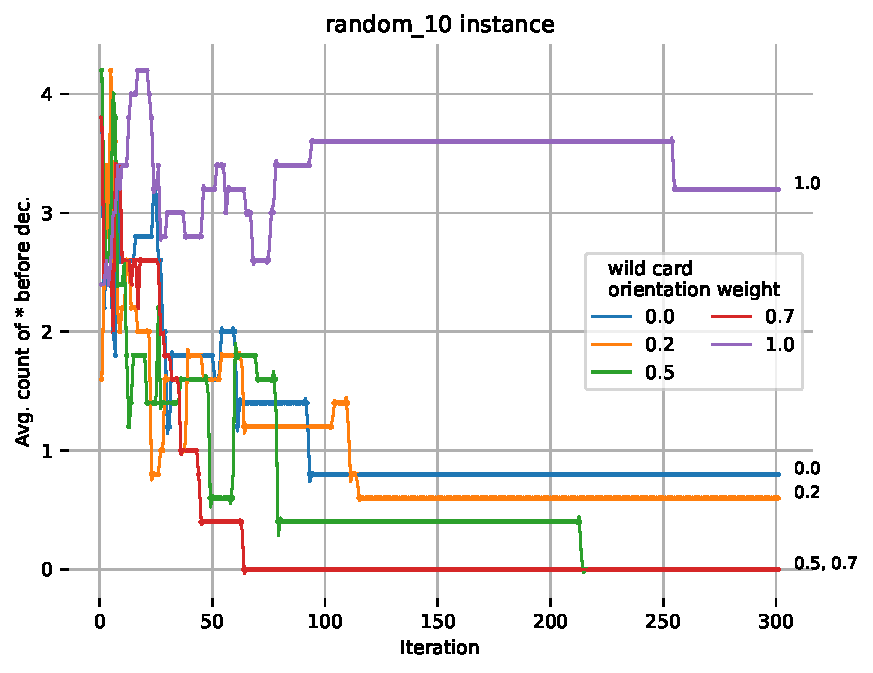
\includegraphics[width=1\textwidth]{hyperparameters/orientation_weights_wildcard_cut_type_spread_random_10}\label{subfig:hyperparameters-orientation-weights-wildcard-cut-type-spread-random-10}}

    \subfloat{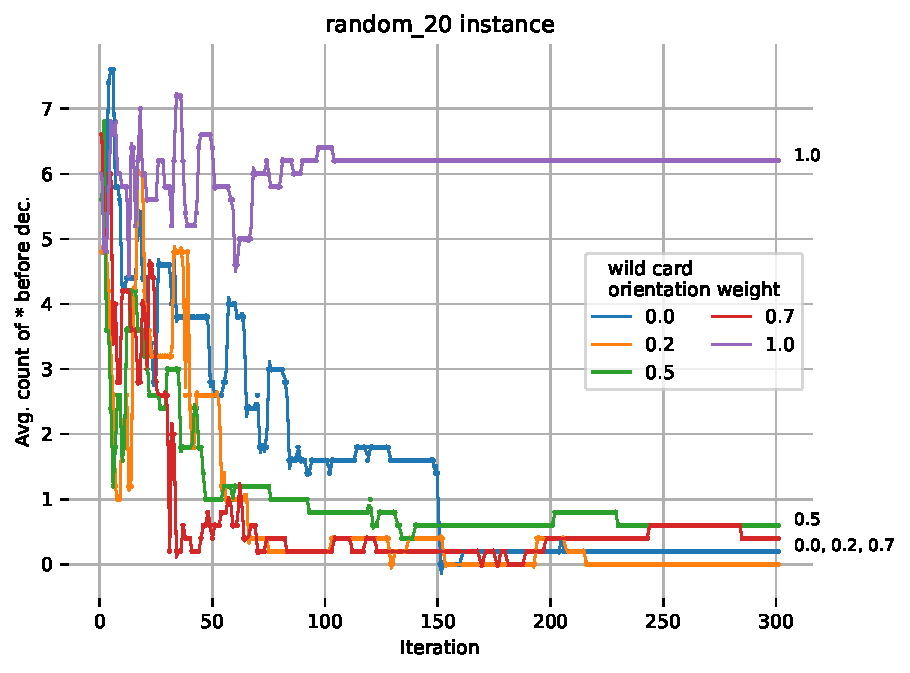
\includegraphics[width=1\textwidth]{hyperparameters/orientation_weights_wildcard_cut_type_spread_random_20}\label{subfig:hyperparameters-orientation-weights-wildcard-cut-type-spread-random-20}}
    \cprotect\caption[Testing wildcard spread]
    {Testing wildcard spread at two random instances.
    Each iteration shows average count of wildcard cut type $*$ at best individual for different values of wild card orientation weights.
    Hyperparameter \verb|maximumWildCardCount| is 1.}
    \label{fig:hyperparameters-orientation-weights-wildcard-cut-type-spread}%
\end{figure}
%    \end{landscape}
%    \clearpage% Flush page
%}

%\afterpage{%
%    \clearpage% Flush earlier floats (otherwise order might not be correct)
%    \begin{landscape}% Landscape page
\begin{figure}
    \centering
    \subfloat{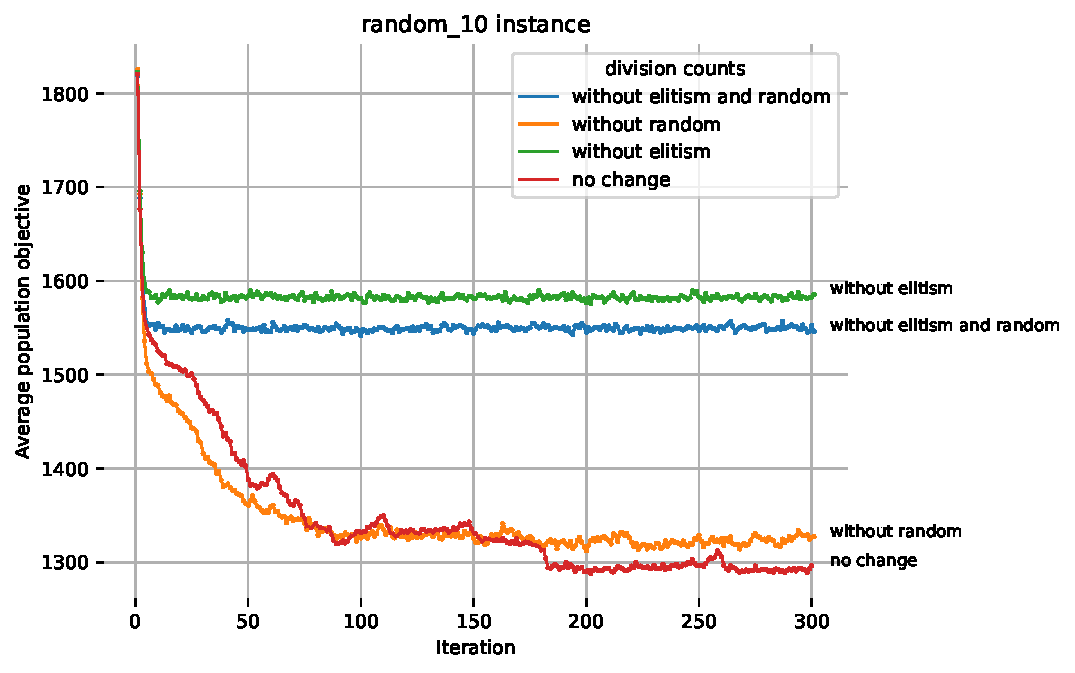
\includegraphics[width=1.1\textwidth]{hyperparameters/population_division_counts_random_10}\label{subfig:hyperparameters-population-division-counts-random-10}}

    \subfloat{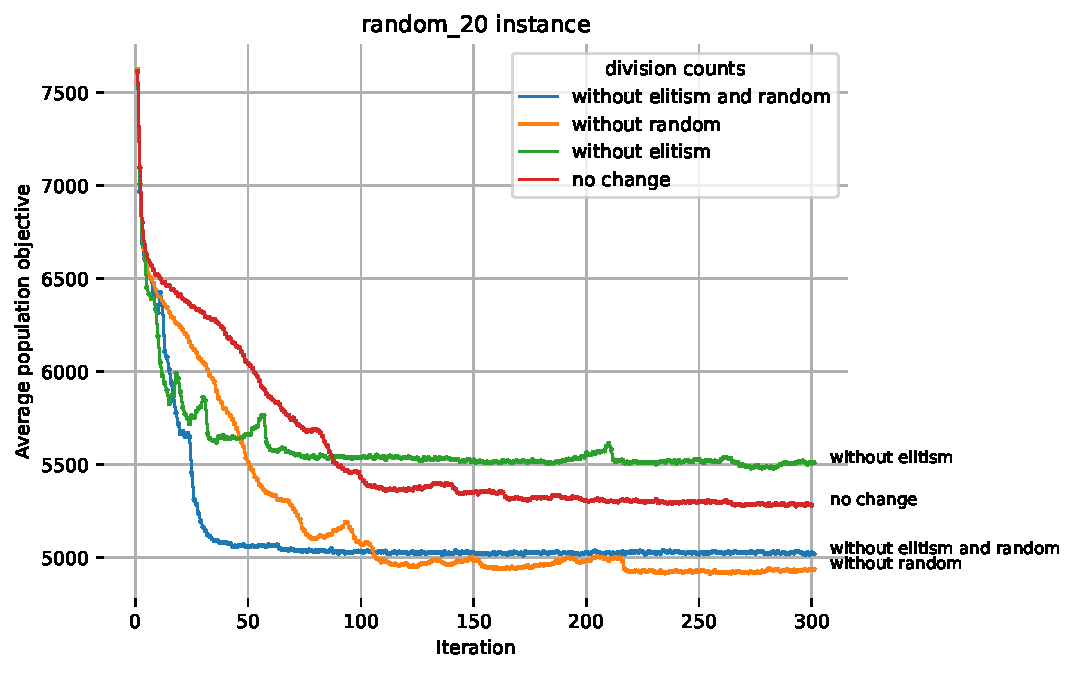
\includegraphics[width=1.1\textwidth]{hyperparameters/population_division_counts_random_20}\label{subfig:hyperparameters-population-division-counts-random-20}}
    \caption[Testing population division counts]
    {Testing population division counts at two random instances.
    Four variants are displayed. First does not use elitism, second does not inject random individuals, third combines first and second,
        and the last does not make any change to the population division counts as described in listing~\ref{lst:computation-submission-dataset}.}
    \label{fig:hyperparameters-population-division-counts}%
\end{figure}
%    \end{landscape}
%    \clearpage% Flush page
%}

\afterpage{%
    \clearpage% Flush earlier floats (otherwise order might not be correct)
    \begin{landscape}% Landscape page
        \begin{figure}
            \centering
            \subfloat{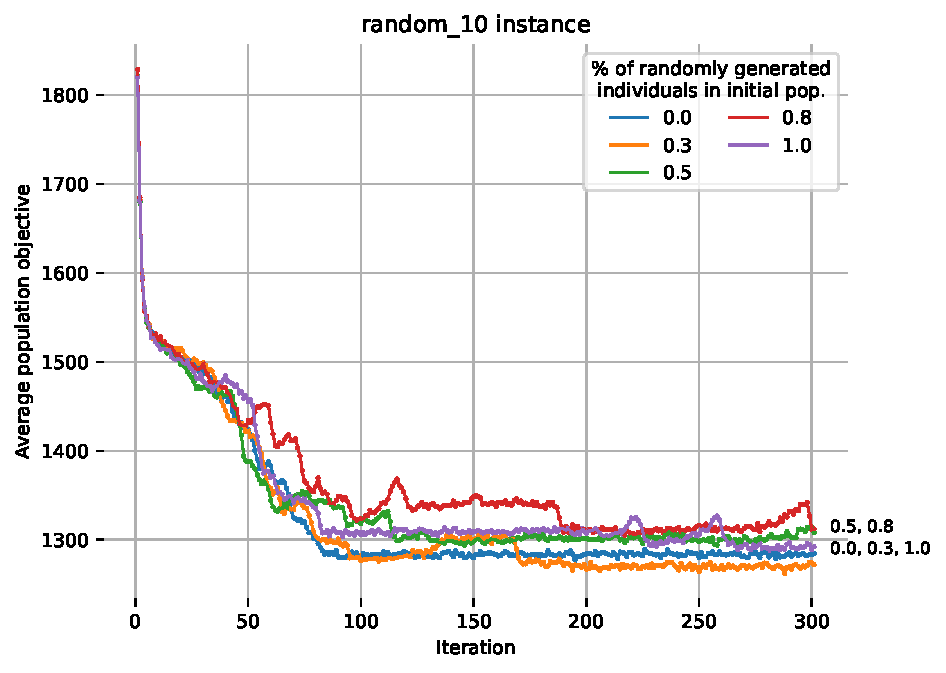
\includegraphics[width=0.8\textwidth]{hyperparameters/initial_population_division_counts_random_10}\label{subfig:hyperparameters-initial-population-division-counts-random-10}}
            \subfloat{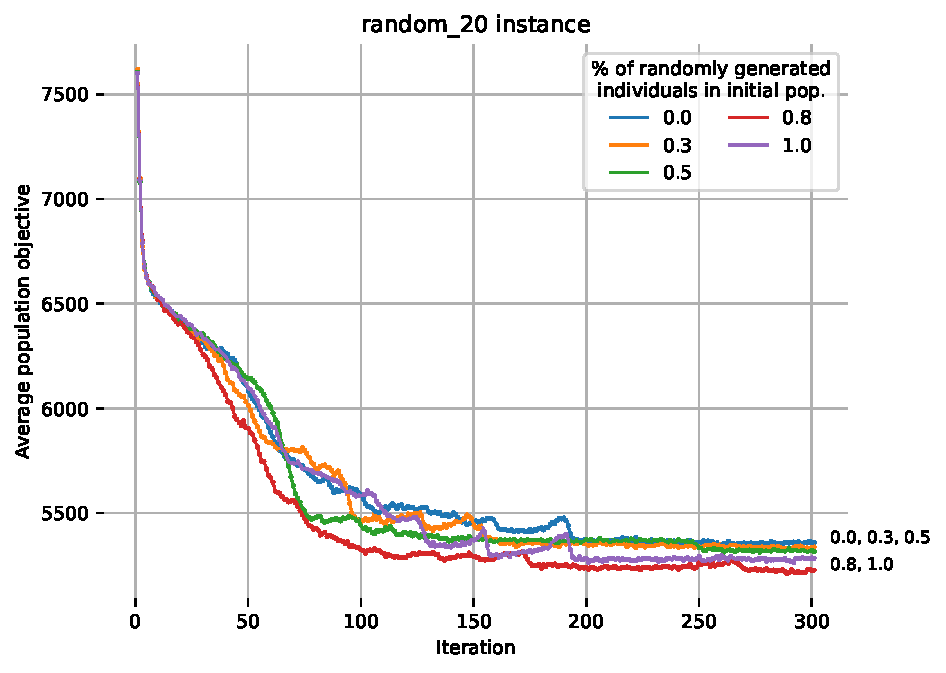
\includegraphics[width=0.8\textwidth]{hyperparameters/initial_population_division_counts_random_20}\label{subfig:hyperparameters-initial-population-division-counts-random-20}}
            \caption[Testing initial population division counts]
            {Testing initial population division counts at two random instances.
            Initial population consists of randomly generated and greedily generated individuals (left part of fig.~\ref{fig:population-schema}).}
            \label{fig:hyperparameters-initial-population-division-counts}%
        \end{figure}
    \end{landscape}
    \clearpage% Flush page
}

\afterpage{%
    \clearpage% Flush earlier floats (otherwise order might not be correct)
    \begin{landscape}% Landscape page
        \begin{figure}
            \centering
            \subfloat{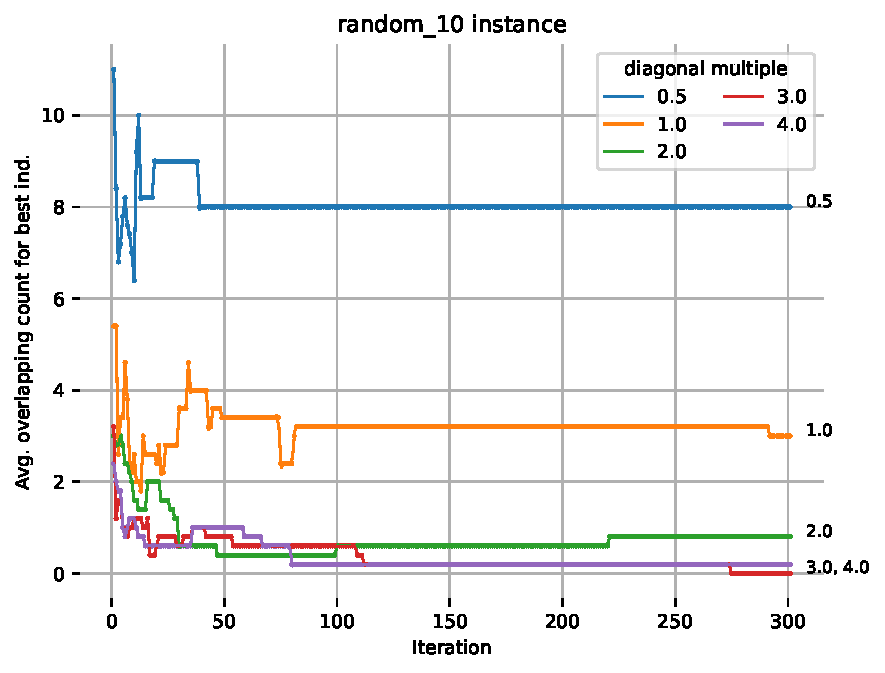
\includegraphics[width=0.8\textwidth]{hyperparameters/overlapping_penalization_constant_random_10}\label{subfig:hyperparameters-overlapping-penalization-constant-random-10}}
            \subfloat{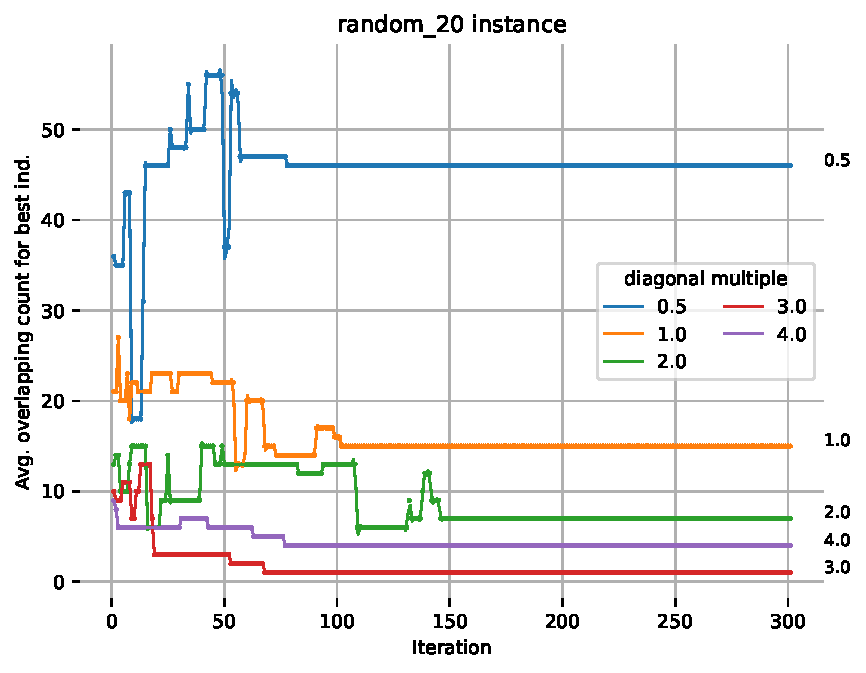
\includegraphics[width=0.8\textwidth]{hyperparameters/overlapping_penalization_constant_random_20}\label{subfig:hyperparameters-overlapping-penalization-constant-random-20}}
            \caption[Testing overlapping penalization constant]
            {Testing overlapping penalization constant $\lambda$ (eq.~\ref{eq:objective}) at two random instances.
            It is determined as $kD$, where $k$ is diagonal multiple and $D$ is the length of a diagonal in a layout.
            Graps show the average averlapping count for best individual at each iteration.}
            \label{fig:hyperparameters-overlapping-penalization-constant}%
        \end{figure}
    \end{landscape}
    \clearpage% Flush page
}

\afterpage{%
    \clearpage% Flush earlier floats (otherwise order might not be correct)
    \begin{landscape}% Landscape page
        \begin{figure}
            \centering
            \subfloat{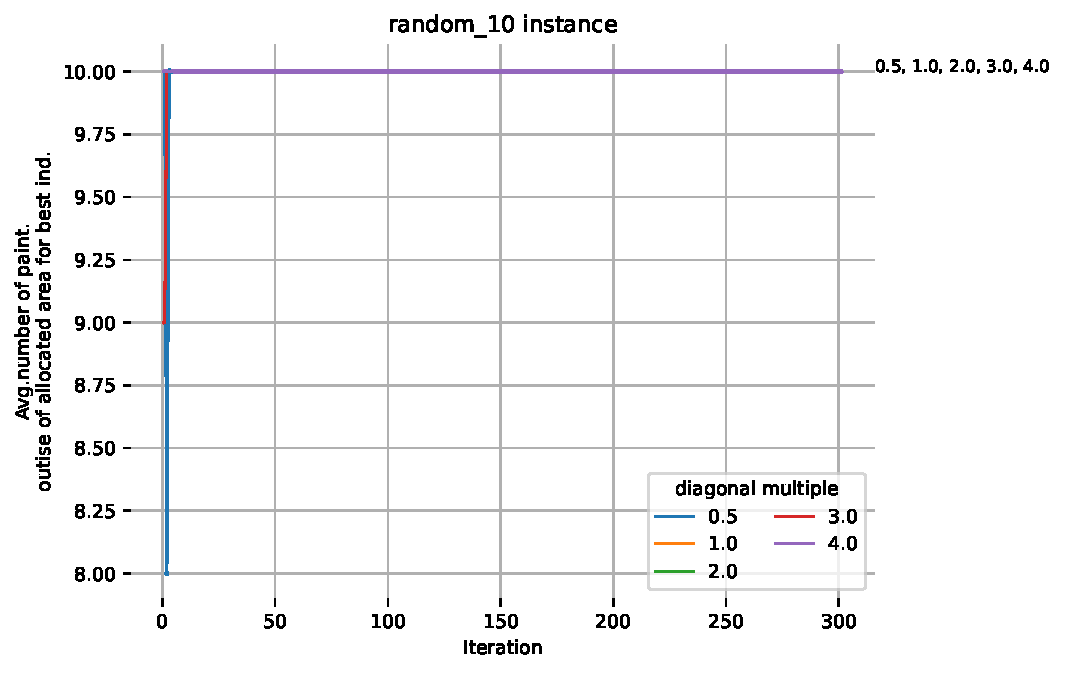
\includegraphics[width=0.8\textwidth]{hyperparameters/outside_of_allocated_area_penalization_constant_random_10}\label{subfig:hyperparameters-outside-of-allocated-area-penalization-constant-random-10}}
            \subfloat{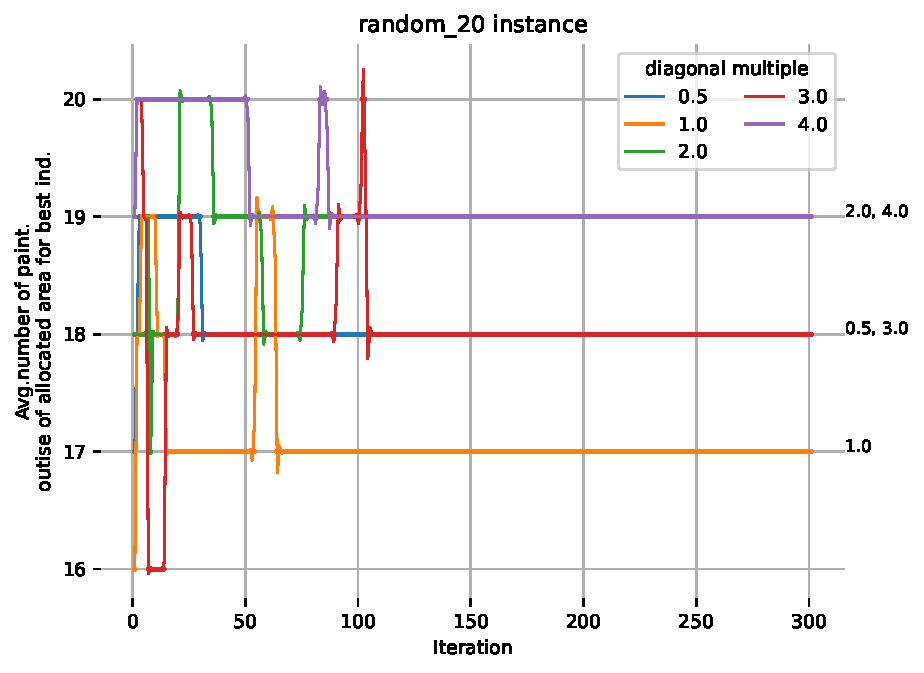
\includegraphics[width=0.8\textwidth]{hyperparameters/outside_of_allocated_area_penalization_constant_random_20}\label{subfig:hyperparameters-outside-of-allocated-area-penalization-constant-random-20}}
            \caption[Testing outside of allocated area penalization constant]
            {Testing outside of allocated area penalization constant $\gamma$ (eq.~\ref{eq:objective}) at two random instances.
            It is determined as $kD$, where $k$ is diagonal multiple and $D$ is the length of a diagonal in a layout.
            Graps show the average number of paintings that are placed outside of their allocated are for best individual at each iteration.}
            \label{fig:hyperparameters-outside-of-allocated-area-penalization-constant}%
        \end{figure}
    \end{landscape}
    \clearpage% Flush page
}

